\documentclass{beamer}

\usepackage[utf8]{inputenc}
\usepackage[T1]{fontenc}
\usepackage[slovene]{babel}
\usepackage{lmodern}
\usepackage{array}
\usepackage{tikz}

\usetheme{Berlin}
\usecolortheme{default}
\useinnertheme[shadows]{rounded}
\useoutertheme{infolines}
\beamertemplatenavigationsymbolsempty

% pisava
\usepackage{palatino}
\usefonttheme{serif}

\newtheorem{definicija}{Definicija}
\newtheorem{izrek}{Izrek}
\newtheorem{trditev}{Trditev}
\newtheorem{domneva}{Domneva}
\newtheorem{lema1}{Lema 1}
\newtheorem{lema2}{Lema 2}
\newtheorem{lema3}{Lema 3}
\newtheorem{lema4}{Lema 4}

\def\N{\mathbb{N}}
\def\Z{\mathbb{Z}}
\def\Q{\mathbb{Q}}
\def\R{\mathbb{R}}


\newenvironment{dokaz}{
   \begin{proof}      
}{
   \end{proof}
}

\begin{document}

% ===================================================================

\title{Porazdelitev praštevil}
%\subtitle{Uporaba paketa beamer}
\author{Matevž Miščič}
\institute[FMF]{Fakulteta za matematiko in fiziko}
\date{21. 8. 2023}
\begin{frame}
   \titlepage
\end{frame}

% ===================================================================

\section{Praštevila}
\begin{frame}
    \frametitle{Praštevila}
    \begin{definicija}
        \textbf{Praštevilo} je naravno število, ki ima natanko dva delitelja.

        Naravno število, ki ima vsaj tri delitelje, imejujemo \textbf{sestavljeno število}.
    \end{definicija}
    \pause
    \medskip
    \begin{exampleblock}{Zgled}
        Prvih nekaj praštevil je $2, 3, 5, 7, 11, 13, \ldots$.

        Število $6$ je sestavljeno število, ker ima štiri delitelje: $1, 2, 3, 6$.
    \end{exampleblock}
 \end{frame}

% -------------------------------------------------------------------

\begin{frame}
    \begin{trditev}
        Vsako naravno število, večje od $1$, se da zapisati kot produkt števil.
    \end{trditev}
    \bigskip
    \pause
    \begin{trditev}
        Praštevil je neskončno mnogo.
    \end{trditev}
\end{frame}

% -------------------------------------------------------------------

\section{Praštevilski izrek}
\begin{frame}
    \frametitle{Praštevilski izrek}
    Med večjimi števili so praštevila bolj redka.
    \medskip
    \begin{definicija}
        Za naravno število $n \in \N$ s \textbf{$\pi(n)$} označimo število praštevil manjših ali enakih $n$.
    \end{definicija}
    \medskip
    Zanima nas, kako raste funkcija $\pi$.
\end{frame}

% -------------------------------------------------------------------

\begin{frame}
    \centering
    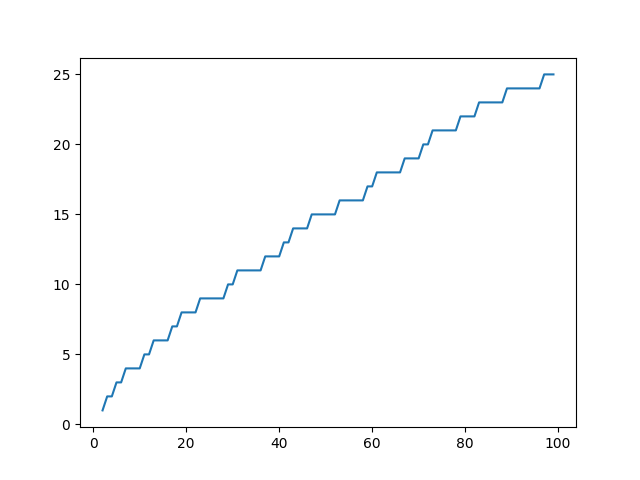
\includegraphics[height=0.95\textheight]{pi.png}
\end{frame}

% -------------------------------------------------------------------

\begin{frame}
    \begin{izrek}[Čebišov]
        Obstajata pozitivni realni števili $A, B > 0$, da za vsak $n \in \N$ velja $$A\frac{n}{\log{n}} < \pi(n) < B\frac{n}{\log{n}}.$$
    \end{izrek}
\end{frame}

% -------------------------------------------------------------------

\begin{frame}
    \centering
    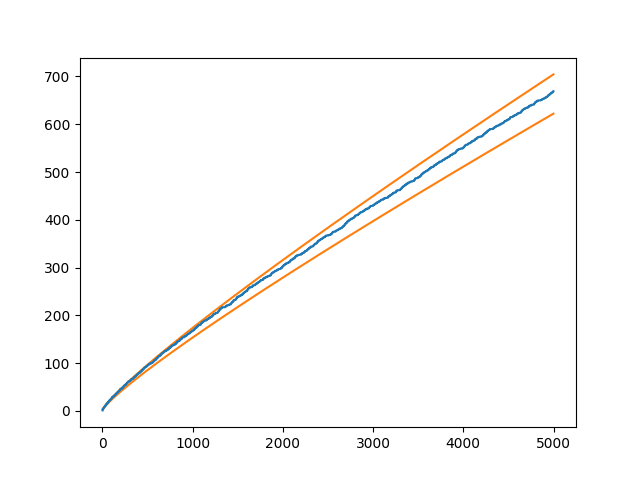
\includegraphics[height=0.95\textheight]{cebisov.png}
\end{frame}

% -------------------------------------------------------------------

\begin{frame}
    \begin{izrek}[Praštevilski izrek]
        Velja $$\lim_{n \rightarrow \infty} \frac{\pi(n)}{n / \log{n}} = 1.$$
    \end{izrek}
\end{frame}

% -------------------------------------------------------------------

\begin{frame}
    \centering
    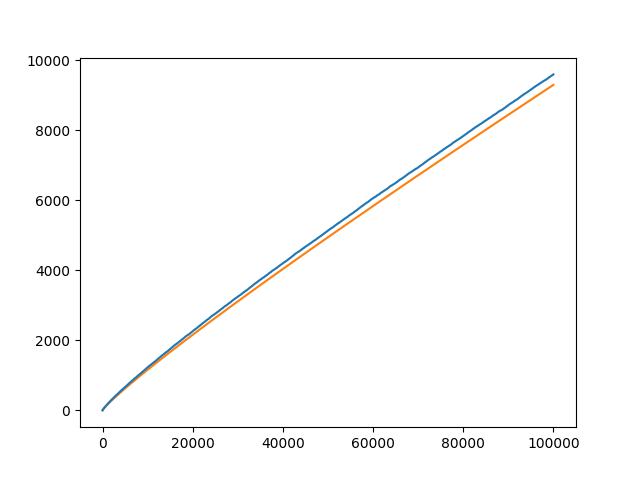
\includegraphics[height=0.95\textheight]{prime_number_theorem.png}
\end{frame}

% ===================================================================

\section{Praštevila v aritmetičnih zaporedjih}
\begin{frame}
    \frametitle{Praštevila v aritmetičnih zaporedjih}
    \begin{izrek}[Dirichlet]
        Naj bosta $a, b \in \N$ tuji si števili. Potem je med členi zaporedja $an + b, n \in \N$ neskončno praštevil.
    \end{izrek}
    \pause
    \begin{exampleblock}{Zgled}
        Če je $a = 3$ in $b = 6$, dobimo aritmetično zaporedje $9, 12, 15, 18, 21, 24, \ldots$. V tem zaporedju so vsi členi deljivi s $3$, ki je največji skupni delitelj $a$ in $b$.
        \medskip
        Če je $a = 8$ in $b = 3$, dobimo zaporedje $11, 14, 17, 20, 23, 26, 29, \ldots$. Od tega so $11, 17, 23, 29$ praštevila. Po Dirichletovem izreku obstaja neskončno praštevilskih členov tega zaporedja.
    \end{exampleblock}
\end{frame}

% -------------------------------------------------------------------

\begin{frame}
    \begin{trditev}
        Med števili oblike $6n + 5$ je neskončno praštevil.
    \end{trditev}
\end{frame}

% ===================================================================

\section{Razmaki med praštevili}
\begin{frame}
    \frametitle{Razmaki med praštevili}
    \begin{trditev}
        Obstajajo poljubno veliki bloki zaporednih naravnih števil, ki so vsa sestavljena števila.
    \end{trditev}
    \medskip
    Po praštevilskem izreku je povprečen razmak med preštevili manjšimi od $n$ približno $\log{n}$. Razmaki torej postajajo vse večji.
\end{frame}

% -------------------------------------------------------------------

\begin{frame}
    \begin{definicija}
        \textbf{Praštevilski dvojček} je par praštevil $(p, q)$, za katerega velja $q - p = 2$.
    \end{definicija}
    \pause
    \medskip
    \begin{exampleblock}{Zgled}
        Primeri praštevilskih dvojčkov so $(3, 5), (5, 7), (9, 11), (11, 13)$.
    \end{exampleblock}
    \pause
    \medskip
    \begin{domneva}
        Ali obstaja neskončno praštevilskih dvojčkov?
    \end{domneva}   
\end{frame}

% -------------------------------------------------------------------

\section{Bertrandov postulat}
\begin{frame}
    \frametitle{Bertrandov postulat}
    \begin{izrek}
        Za vsako naravno število $n \in \N$ obstaja praštevilo $p$ za katero velja $n \leq p \leq 2n$.
    \end{izrek}
    \medskip
    Izrek je prvi dokazal Pafnuti Čebišov leta 1850, mi pa si bomo ogledali enostavnejši dokaz, ki ga je podal Paul Erd\H{o}s leta 1932.
\end{frame}

% -------------------------------------------------------------------

\begin{frame}
    \frametitle{Paul Erd\H{o}s}
    \centering
    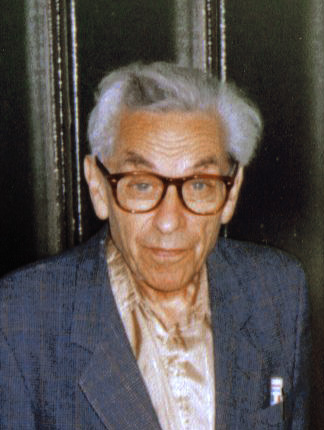
\includegraphics[height=0.8\textheight]{erdos.jpg}
\end{frame}

% -------------------------------------------------------------------

\begin{frame}
    \begin{definicija} % povej kaj je fakulteta
        \textbf{Centralni binomski koeficient} je število $$C_n = \binom{2n}{n} = \frac{(2n)!}{n!^2}.$$
    \end{definicija}
    \pause
    \medskip
    \begin{lema1}
        \label{lema1}
        Za vsako naravno število $n$ velja $\frac{4^n}{2n} \leq C_n$.
    \end{lema1}
    \pause
    \medskip
    \begin{lema2}
        \label{lema2}
        Za vsako naravno število $n \in \N$ za praštevilski razcep $C_n = p_1^{a_1} \cdots p_r^{a_r}$ velja $p_i^{a_i} \leq 2n$ za vsak $i = 1,\ldots,r$. 
    \end{lema2}
\end{frame}

% -------------------------------------------------------------------

\begin{frame}
    \begin{lema3}
        \label{lema3}
        Za vsako naravno število $n \in \N$ in praštevilo $p \neq 2$ z $\frac{2n}{3} < p < n$ velja, da $p$ ne deli $C_n$. 
    \end{lema3}
    \pause
    \medskip
    \begin{definicija}
        Za naravno število $n \in \N$ definirajmo \textbf{$n$-to primorielo} kot produkt vseh praštevil manjših ali enakih $n$ in jo označimo z $n\#$.
    \end{definicija}
    \pause
    \medskip
    \begin{lema4}
        \label{lema4}
        Za vsako naravno število $n \in \N$ velja $n\# < 4^n$. 
    \end{lema4}
\end{frame}

\end{document}